
%==========================================================================

\begin{frame}[fragile]

  {\Huge Organizational}

  \vspace{10pt}

  \textbf{Content:}
  \begin{itemize}
    \item Linux Foundation
    \item{\texttt{develop} Branch}
    \item Targetting C++20 for Kokkos 5.0
  \end{itemize}

\end{frame}

%==========================================================================

\begin{frame}[fragile]{High Performance Software Foundation}
\begin{center}
\textbf{Kokkos is now a member of the}

\vspace{0.2cm}
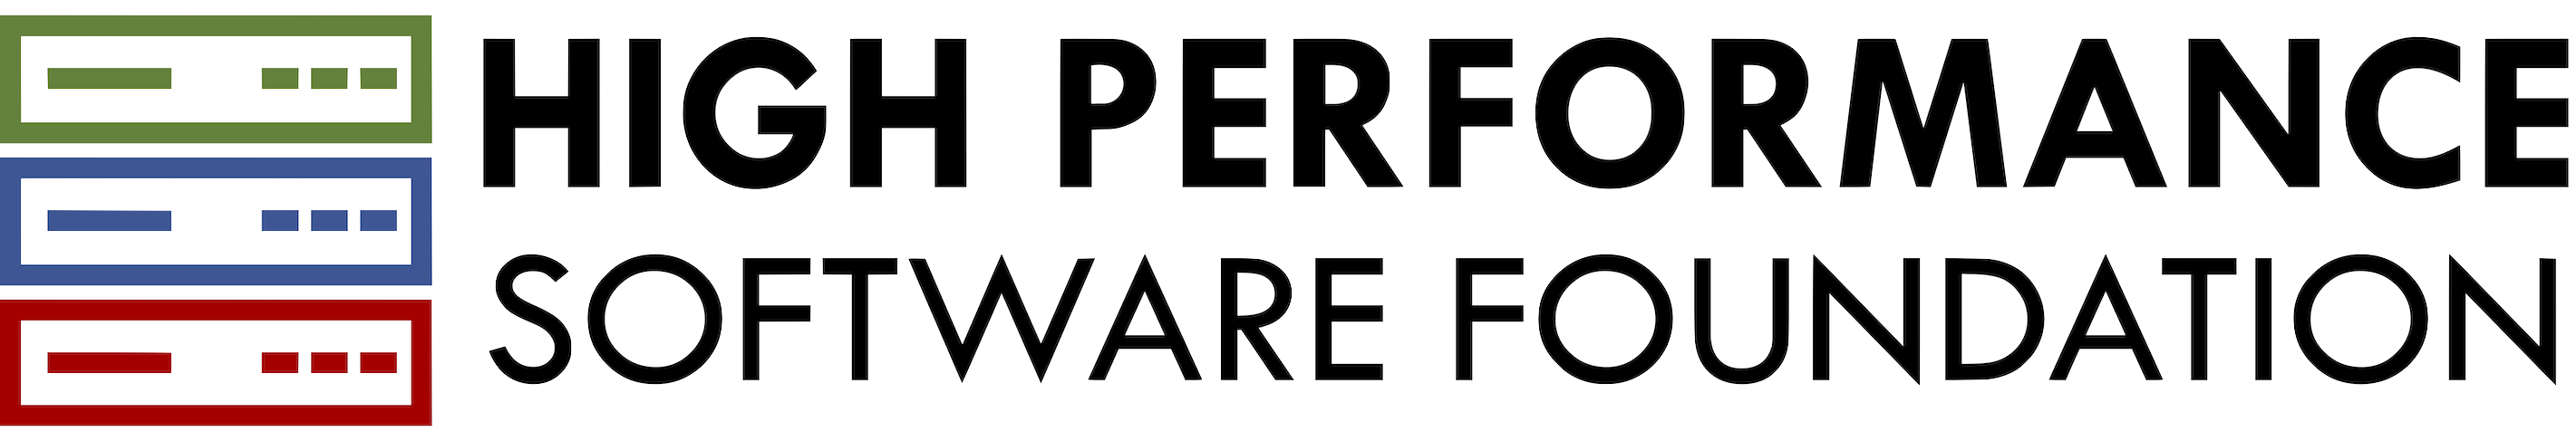
\includegraphics[width=.45\textwidth]{4_4/hpsf-logo}

\vspace{0.2cm}
\textit{HPSF supports the community development of key HPC projects}
\end{center}

\textit{Member Organizations}
\begin{itemize}
  \item{Labs: LLNL, SNL, ORNL, LANL, ANL, CEA}
  \item{Industry: HPE, AWS, NVIDIA, Intel, AMD, Kitware}
  \item{Academia: U-Oregon, U-Maryland, CDAC}
\end{itemize}

\textit{Member Projects}
\begin{itemize}
  \item Spack, Kokkos, Trilinos, AMReX, WarpX, Viskores, HPCToolkit, E4S, Charliecloud, Apptainer
\end{itemize}
\end{frame}

\begin{frame}[fragile]{High Performance Software Foundation}
\textit{What will HPSF do?}
\begin{itemize}
  \item Provide framework for collaboration on common community concerns (working groups for CI, software security, training etc.)
  \item Help organize user-group meetings and trainings
  \item Pay for some community infrastructure (e.g. webpage, CI, Slack?)
\end{itemize}

\textit{Getting Involved:}
\begin{itemize}
  \item Talk to us - Christian, Damien and Julien are all active in HPSF
  \item We are still in bring-up phase: working groups are not yet constituted
\end{itemize}
\end{frame}

\begin{frame}[fragile]{Release Mechanisms}
\textbf{develop} is now the default branch of Kokkos Core and Kernels
\begin{itemize}
  \item{Switched with 4.3 release}
  \item{master branch is deprecated - still updated to 4.4 right now}
\end{itemize}

Started to publish signed release artifacts
\begin{itemize}
  \item{Release page: \url{https://github.com/kokkos/kokkos/releases/latest}}
  \item \textbf{Source distributions}: source archives uploaded by the Kokkos team
  \item \textbf{Summary files}: Hashes and keys to verify integrity of hash
  \item \textbf{Assets:} All the files. Note: \textbf{Source code (zip/tar.gz)} are GitHub autogenerated and do not promise a stable checksum
\end{itemize}
\end{frame}

\begin{frame}[fragile]{Verify integrity}
Commands for 4.4:
\begin{code}
KOKKOS_RELEASES=https://github.com/kokkos/kokkos/releases
wget $\$${KOKKOS_RELEASES}/download/4.4.00/kokkos-4.4.00.tar.gz
wget $\$${KOKKOS_RELEASES}/download/4.4.00/kokkos-4.4.00-SHA-256.txt
wget $\$${KOKKOS_RELEASES}/download/4.4.00/kokkos-4.4.00-SHA-256.txt.asc
wget https://kokkos.org/downloads/signing-keys/dalg24.asc
gpg --import dalg24.asc
gpg --verify kokkos-4.4.00-SHA-256.txt.asc
grep kokkos-4.4.00.tar.gz kokkos-4.4.00-SHA-256.txt | sha256sum -c
\end{code}

Relevant Output:
\begin{code}
gpg --verify kokkos-4.4.00-SHA-256.txt.asc
  ...
  gpg: Good signature from "Damien Lebrun-Grandie <dalg24@gmail.com>" \[unknown\]
  gpg: WARNING: This key is not certified with a trusted signature!
  ...
grep kokkos-4.4.00.tar.gz kokkos-4.4.00-SHA-256.txt | sha256sum -c
  kokkos-4.4.00.tar.gz: OK
\end{code}
\end{frame}

\begin{frame}[fragile]{Kokkos 5 and ISO C++20}
\begin{center}
\textbf{Kokkos 5 is comming Summer 2025}

\vspace{0.5cm}
\textbf{We will require C++20!}
\end{center}

\textit{Start preparing now:}
\begin{itemize}
  \item{Check availability of compilers on your systems}
  \item{Test with C++20 enabled: start with a CPU build}
  \item{Minimum Compiler requirements will change (more details later)}
\end{itemize}

\vspace{0.5cm}
\begin{center}
\textit{Nothing wrong for your project to require C++20 now if you feel ready!}
\end{center}
\end{frame}

